\section{Введение}
\subsection{Теоретические сведения}

\textbf{Цель работы:}
изучение работы высокочувствительного зеркального галь­ ванометра магнитоэлектрической системы в режимах измерения постоян­ного тока и электрического заряда.

\textbf{В работе используются:}
зеркальный гальванометр с осветителем и шка­лой, источник постоянного напряжения, делитель напряжения, магазин со­противлений, эталонный конденсатор, вольтметр, переключатель, ключи, линейка.

\begin{wrapfigure}{r}{0.5\linewidth} % l - слева, r - справа, с - центр
\centering %выравнивание по центру
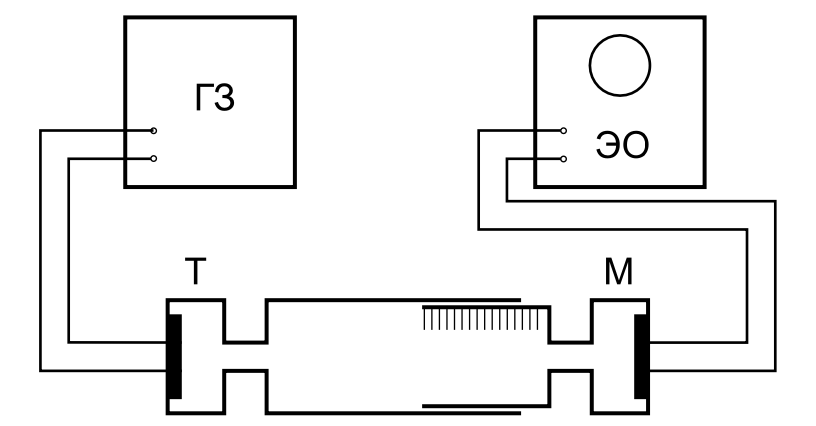
\includegraphics[width=0.5\linewidth,center]{p1.png}
\caption{Рамки с током в магнитном поле} % подрисуночная подпись
\label{pic:my} %метка для ссылки по тексту
\end{wrapfigure}

\textit{Баллистическим гальванометром} называют электроизмерительный прибор магнитоэлектрической системы, отличающийся высокой чув­ ствительностью к току и сравнительно большим периодом колебаний подвижной системы (рамки).

Главной частью баллистического гальвано­метра является подвешенная на вертикальной нити рамка, помещённая в поле постоянного магнита. Вырез цилиндрической формы в по­ люсах магнита и ферромагнитный цилиндр на оси системы делают поле в зазоре радиаль­ным (рис. 1). Скреплённое с рамкой зеркаль­ це служит для измерения угла поворота рам­ки. К рамке прикреплён полый цилиндр, ко­торый сильно увеличивает момент инерции и, следовательно, период колебаний подвижной системы, не очень её утяжеляя. Магнит и по­ движная система заключены в защитный ко­жух. В баллистических гальванометрах
при­меняют сильные постоянные магниты и рамки с большим количеством витков, подвешенные на тонких нитях с малой упругостью.

Уравение колебаний рамки в магнитном поле:
\begin{equation}
    \ddot{\varphi} + 2 \gamma\dot{\varphi} + \omega_0^2\varphi = KI,
    \label{equ:ddotvarphi}
\end{equation}
где $ 2\gamma = \dfrac{(BSN)^2}{JR_\Sigma}$, $\omega_0^2 = \dfrac{D}{J}$, $K = \dfrac{BSN}{J}$.

\subsection{Определение динамической постоянной гальванометра}

Схема для исследования гальванометра в стационарном режиме представлена на рис. 2. Постоянное напряжение $U$ снимается с блока питания и измеряется вольтметром $V$ . Ключ $K_3$ позволяет менять на­ правление тока через гальванометр Г, делитель напряжения — менять величину тока в широких пределах. Ключ $K_2$ служит для включения гальванометра, кнопка $K_1$ — для его успокоения. Магазин сопротивле­ ний $R$ позволяет менять режим работы гальванометра от колебательно­го до апериодического.

\begin{figure}[h]
    \centering
    \includegraphics*[width = 0.75\linewidth]{p2.png}
    \caption{Схема установки для работы гальванометра в стационарном режиме}
    \label{pic:p2}
\end{figure}

Если в схеме на рис. \ref{pic:p2} будет протекать постоянный ток, то в (\ref{equ:ddotvarphi}) динамическую постоянную для гальванометра, используя угол поворота, можно определить формулой
\begin{equation}
    C_1 = \frac I \varphi = \frac{2aI}{x},
    \label{equ:C_1}
\end{equation}
где $a$ -- расстояние между гальванометром и линейкой, x -- отклонение зайчика.

\subsection{Определение критического сопротивления гальванометра}

При затухающих колебаниях вводится логарифмический де4кремент затухания:
\begin{equation}
    \Theta = \gamma T_1 = \ln\frac {x_n} {x_{n+1}}.
    \label{equ:Theta}
\end{equation}

В таком случае можно опрделить критическое сопротивление по формуле:
\begin{equation}
    R_\text{кр} = \frac{R+R_0}{\sqrt{\left(\frac{2\pi}{\Theta}\right)^2 + 1}} - R_0
    \label{equ:Rkr}
\end{equation}

\subsection{Определение баллистической постоянной и критического сопротивления гальванометра, работающего в баллистическим режиме}
Для изучения работы гальванометра в режиме измерения заряда (в баллистическом режиме), используется схема, представленная на рис. \ref{pic:p3}. Система ключей устроена так, что нормально ключ $K_2$ замкнут, а ключи $K_3$ и $K_4$ разомкнуты. При нажатии на кнопку $K_0$ сначала раз­ мыкается ключ $K_2$, затем замыкается $K_3$ и через некоторое время — $K_4$. При нормальном положении кнопки $K_0$ конденсатор $C$ заряжается до напряжения $U_C$ и получает заряд $q$:

\begin{figure}[h]
    \centering
    \includegraphics*[width = 0.75\linewidth]{p3.png}
    \caption{Схема установки для определения баллистической постоянной}
    \label{pic:p3}
\end{figure}

\begin{equation*}
    U_C = \frac{R_1}{R_2} U_0, \text{   } q = C U_C = C \frac{R_1}{R_2} U_0
\end{equation*}

Первый отброс зайчика $\varphi_{max}$ после нажатия на кнопку $K_0$ зависит от сопротивления внешней цепи, подключённой к гальванометру. Для опре­ деления $R_\text{кр}$ используется то обстоятельство, что в критическом режиме максимальное отклонение зайчика в $e$ раз меньше, чем у гальванометра без затухания.

Величину максимального отклонения рамки гальванометра без затухания $\varphi^\text{св}_{max}$ можно, однако, рассчитать, если при разомкнутой цепи измерить реальное максимальное отклонение рамки $\varphi_0$ и логарифми­ческий декремент затухания $\Theta_0$:
\begin{equation*}
    \varphi_0 = \varphi(T_1/4) = \varphi^\text{св}_{max} e^{-\Theta/4},
\end{equation*}
так что максимальное отклонение рамки гальванометра без затухания
\begin{equation}
    varphi^\text{св}_{max} = \varphi_0 e^{-\Theta/4} \approx \varphi_0 \left(1 + \frac{\Theta_0}{4}\right)
\end{equation}

Баллистическая постоянная гальванометра $C_\text{кр}$ $[\frac{\text{Кл}}{\text{мм/м}}]$определяется при критическом сопротивлении ($R = R_\text{кр}$):
\begin{equation}
    C^\text{кр}_q = \frac{q}{\varphi^\text{кр}_{max}} = 2a\frac{R_1}{R_2} \frac{CU_0}{x^\text{кр}_{max}}.
    \label{equ:Ckrq}
\end{equation}
